\documentclass{ximera}

\title{Verschil van vectoren}
%\author{Daan Lipkens} %van wiskudne op maat Sint-Pieterscollege

\begin{document}
\begin{abstract}

\end{abstract}
\maketitle



Net zoals bij getallen $5 - 3 = 5 + (-3)$, kan je ook bij vectoren een verschil schrijven als een som met de tegengestelde vector: 

\[ \vec{c} = \vec{a} - \vec{b} = \vec{a} + (-\vec{b}) \]

Om $\vec{c}$ te vinden moeten $\vec{a}$ en $-\vec{b}$ dus worden samengesteld. Het verschil van de getallen acht en vijf is gelijk aan drie. Drie is dus het getal dat je bij vijf moet optellen om acht te bekomen. Op dezelfde manier is het verschil van vectoren $\vec{a}$ en $\vec{b}$ gelijk aan de vector $\vec{c}$ die je bij $\vec{b}$ moet optellen om $\vec{a}$ te bekomen. $\vec{c}$ is dus letterlijk het verschil of 'onderscheid' tussen $\vec{a}$ en $\vec{b}$. 

%---------------------------
% AFBEELDING: Verschil van vectoren
\begin{figure}[ht!]
    \captionsetup{width=0.85\textwidth}
    \begin{center}
        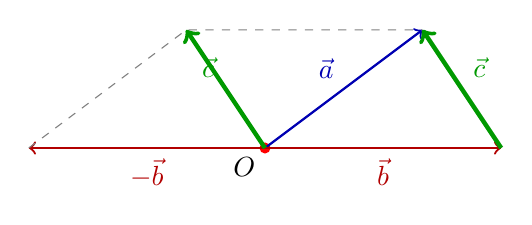
\begin{tikzpicture}[scale=1]
            \coordinate (O) at (0,0);
            \coordinate (A) at (2,1.5);
            \coordinate (B) at (3,0);
            \coordinate (minB) at (-3,0);
            \coordinate (C) at (-1,1.5); % A - B
            
            \fill[red] (O) circle (2pt) node[below left, text=black]{$O$};
            
            \draw[->, thick, blue!70!black] (O) -- (A) node[midway, above left]{$\vec{a}$};
            \draw[->, thick, red!70!black] (O) -- (B) node[midway, below]{$\vec{b}$};
            \draw[->, thick, red!70!black] (O) -- (minB) node[midway, below]{$-\vec{b}$};
            
            % Resultante op oorsprong
            \draw[->, ultra thick, green!60!black] (O) -- (C) node[midway, above left]{$\vec{c}$};
            \draw[dashed, gray] (minB) -- (C) -- (A);
            
            % Resultante tussen koppen
            \draw[->, ultra thick, green!60!black] (B) -- (A) node[midway, above right]{$\vec{c}$};
        \end{tikzpicture}
    \end{center}
    \caption{Het verschil van de vectoren $\vec{a}$ en $\vec{b}$.}
    \label{fig:verschil_vectoren}
\end{figure}
%---------------------------

Grafisch blijkt dat indien $\vec{a}$ en $\vec{b}$ in hetzelfde punt aangrijpen, de verschilvector $\vec{a} - \vec{b}$ gelijk is aan de vector die vertrekt in het eindpunt van $\vec{b}$ en eindigt in het eindpunt van $\vec{a}$.

\end{document}